\subsection{Bot Telegram}
	La componente \textit{bot Telegram} permette di ricevere codici di autenticazione a due fattori, notifiche di alert ed inviare direttamente dei comandi ai singoli dispositivi, per alterarne lo stato.
	\newline
	La componente è stata sviluppata usando JavaScript ed i moduli Axios, HTTP e Telegraf.
	 
\subsubsection{Diagramma delle classi}%%%%%%%%%%%%%%%%%OK
	\begin{figure}[H]
		\centering
		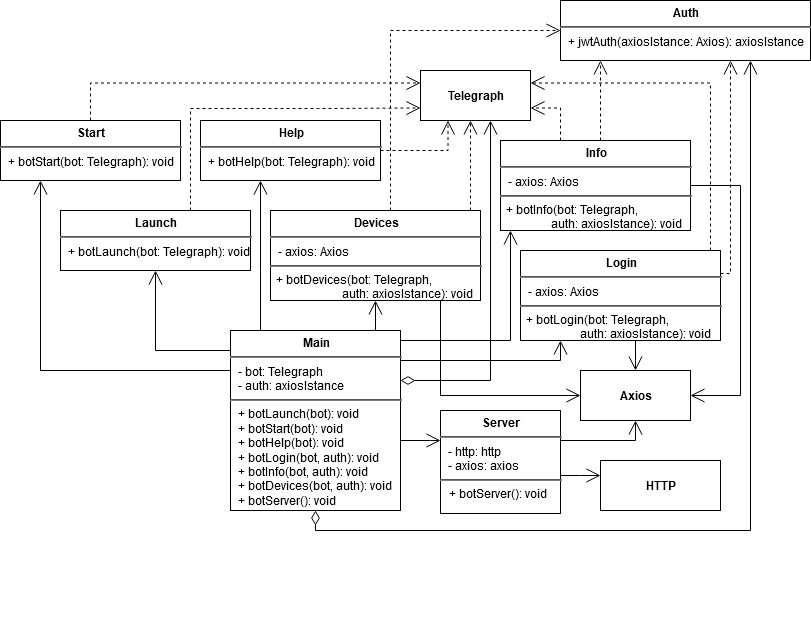
\includegraphics[scale=0.600]{res/images/BOTTELEGRAM/ClassiTelegram.png}
		\caption{Diagramma delle classi della componente bot Telegram}
		\label{Diagramma 19}
	\end{figure}
\subsubsection{Dipendenze esterne}	
	La componente ha tre dipendenze esterne:
	\begin{itemize}
		\item \textbf{Telegraf}, modulo che permette di collegarsi con le API ufficiali di Telegram. Ogni comando ne ha un riferimento. 
		\item \textbf{Axios}, modulo che permette di effettuare richieste POST e GET e di ritornare una risposta. Viene utilizzato da Server, Login e Status per comunicare con le \textit{API} e per inviare uno o più messaggi agli utilizzatori del bot;
		\item \textbf{HTTP}, modulo che permette di creare un server HTTP per restare in ascolto di eventuali richieste. Viene utilizzato da Server per ascoltare eventali richieste delle \textit{API}.    
	\end{itemize}
\subsubsection{Diagramma di sequenza}%%%%%%%%%OK
	\begin{figure}[H]
		\centering
		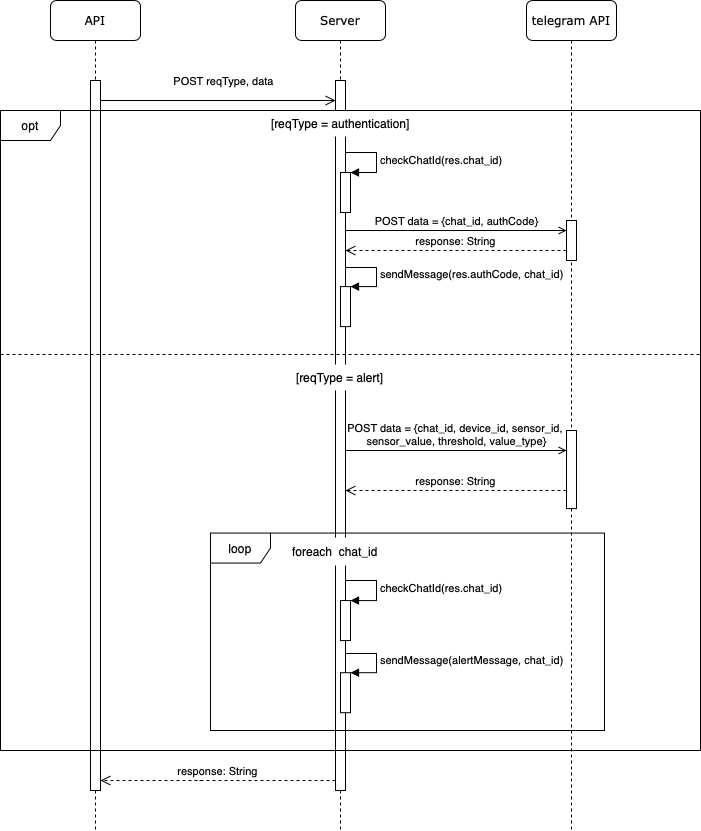
\includegraphics[scale=0.600]{res/images/BOTTELEGRAM/TelegramRichiestaPOST.png}
		\caption{Diagramma di sequenza che riporta la ricezione di una richiesta POST delle \textit{API} all'interno della componente bot Telegram}
		\label{Diagramma 20}
	\end{figure}

	Nel diagramma di sequenza in alto viene mostrata la ricezione di una richiesta POST dalle \textit{API}. La richiesta può essere di due tipologie: 
	\begin{itemize}
		\item authentication, in cui vengono inviati dalle \textit{API} un chat Id ed un codice di autenticazione. Quest'ultimo dovrà poi essere inviato al chat Id specificato per permettere all'utente l'autenticazione sulla webapp;
		\item alert, in cui vengono mandati dalle \textit{API} una lista di chat id ed un insieme di dati che poi andranno composti in un messaggio ed inviati a tutti i chat Id specificati.
	\end{itemize}
\subsubsection{Estensione}
	\paragraph{Inserimento di un nuovo comando}
		Per inserire un nuovo comando all'interno del bot è necessario creare un file .js all'interno della cartella commands. Poichè sarà poi necessario esportare questo comando per poi inserirlo all'interno di main.js l'intestazione del nuovo comando dovrà essere del tipo:
		\begin{verbatim}const botNomeComando = (bot) => {
								bot.command( "nomeComando", (param) => {
							 		...
							 	});
						}; 
		\end{verbatim}	